\chapter{Liga Robocup \label{chap:robocup}}
\section{Opis projektu Robocup \label{sec:opis_robocup}}
	Projekt Robocup, jego idea jak i historia zostały opisane w pracy inżynierskiej \cite{inzynierka}, więcej informacji na temat mistrzost można także znaleźć na oficjalnej stronie projektu
	\mbox{\url{http://www.robocup.org}}. W niniejszej pracy problematyka rozgrywek robotów w piłkę nożną zostanie przedstawiona jedynie skrótowo ze szczególnym uwzględnieniem
	budowy robota wykorzystywanego w lidze na której wzorowano się podczas prac.
	Głównym celem przedsięwzięcia jest stworzenie do 2050 roku drużyny w pełni autonomicznych robotów humanoidalnych zdolnych wygrać rozgrywkę z aktualnymi mistrzami 
	świata.
	Aby osiągnąć zamierzony cel należy połączyć osiągnięcia z różnych dziedzin nauki. Przede wszystkim ważna jest konstrukcja zarówno mechaniczna jak i elektroniczna
	robota. Zawodnik powinien być wyposażony w odpowiedni zestaw czujników umożliwiających osiągnięcie pełnej autonomiczności. 
	Z drugiej strony natomiast należy dysponować funkcjonalnym oprogramowaniem umożliwiającym współpracę wielu robotów.
	Projekt jest realizowany nieprzerwanie od września 1993 roku. Początkowo brali w nim udział jedynie przedstawiciele środowisk naukowych z Japonii.
	Rozgrywki toczone są w kilku niezależnych od siebie ligach.
	Aktualnie wyróżnione zostały nastepujące ligi:
	\begin{itemize}
	\item liga symulacyjna
	\item \emph{Small-size League}
	\item \emph{Middle-size League}
	\item \emph{Standard Platform League }
	\item \emph{Humanoid League}
	\end{itemize}
	Liga symulacyjna jest pewnego rodzaju grą, w której uczestniczące drużyny implentują program decydujący o zachowaniu zawodników.
	Jest ona najstarszą z lig, towarzyszy przedsięwzięciu od samego początku jego istnienia.
	Zachowanie robotów jest symulowane za pomocą programu zwanego \emph{Robocup Soccer Simulator}.

	Kolejną z lig jest \emph{Small-Size League}. W rozgrywkach tej ligi drużyna składa się maksymalnie z pięciu niewielkich robotów, takich jak widoczne na fotografii \ref{fig:F180}. 
	Roboty  nie są jednak w pełni autonomiczne, ponieważ nie
	posiadają własnych sensorów. Algorytm sterujący czerpie informację o~położeniu piłki oraz robotów z kamery
	umieszczonej centralnie nad boiskiem. Lidze tej został poświęcony w całości paragraf \ref{sec:F180}.	
	\begin{figure}[ht]
	\centering
	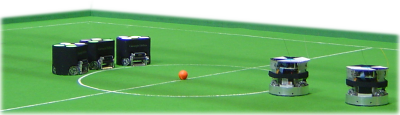
\includegraphics[scale=0.7]{./liga_robocup/F180}
	\caption{ Roboty biorące udział w \emph{Small-Size League}\newline(źródło: \texttt{www.robocup.org})} \label{fig:F180}
	\end{figure}
	
	\emph{Middle-size League} to rozgrywki w pełni autonomicznych robotów. W odróżnieniu od wcześniej omawianej
	ligi małych robotów, globalny system wizyjny jest całkowicie zakazany. Każdy robot jest wyposażony w osobny zestaw czujników wizyjnych.
	Zadaniem zawodników jest reagowanie na sytuację na planszy i koordynowanie swoich działań w zależności od zachowań innych graczy.

	W projekcie wyróżnione są także ligi \emph{Standard Platform League }, czyli rozgrywki piesków \textit{Aibo} konstruowanych przez firmę \textit{Sony} oraz 
	liga robotów humanoidalnych. W tej ostatniej biorę udział roboty przypominające swoją budową ludzi czyli posiadać korpus, nogi, ręce oraz głowę.
	\section{Szczegółowe omówienie ligi Small-size (F180)}
	\subsection{Zasady}
	Zbiór zasad obowiązujący w lidze podlega co roku aktualizacji przez komitet techniczny ligi. Zazwyczaj około
	rok przed kolejnymi mistrzostwami znane są zasady na nich obowiązujące. Początkowo w rozgrywkach wszystkie
	roboty  korzystały  z globalnego systemu wizyjnego, jednak w  trakcie kolejnych zmian w przepisach
	dopuszczono do rozgrywek roboty z własnym systemem wizyjnym, dzięki czemu  zaczęto wykorzystywać także
	rozproszone algorytmy sterowania.
	
	W rozgrywce na boisku o wymiarach 7.4~[m] na 5.4~[m] wyłożonej zielonym dywanem lub wykładziną biorą udział dwie
	drużyny składające się z maksymalnie pięciu robotów. Jeden z robotów może zostać oddelegowany do pełnienia
	funkcji bramkarza, jednak powinno to zostać zgłoszone przed rozpoczęciem meczu. 
	Konstrukcja robota powinna zmieścić się w walcu o średnicy 18~[cm] oraz wysokości 15~[cm]. W przypadku robotów z
	własnymi sensorami wizyjnymi dopuszcza się wysokość do 22.5~[cm]. Robot może być wyposażony w urządzenie do prowadzenia piłki, jednak istnieją pewne ograniczenia dotyczące
	jego budowy oraz stosowania w czasie gry. Mianowicie robot może prowadzić piłkę maksymalnie przez dystans
	50~[cm], po przejechaniu którego powinien albo podać ją innemu zawodnikowi, albo kopnąć przed siebie i dalej ją
	prowadzić. W przeciwnym wypadku sygnalizowane jest przewinienie. Natomiast konstrukcja urządzenia do dryblowania nie może uniemożliwiać kontaktu z piłką zawodnikowi z przeciwnej drużyny.
		
	Rozgrywka jest całkowicie kontrolowana przez arbitra, który czuwa nad tym, aby  regulamin był przestrzegany. Do
	jego zadań należy sygnalizowanie przewinień, zdobytych bramek oraz innych typowych sytuacji na boisku.
	Sędzia ma prawo zmienić swoją decyzje po konsultacjach z asystentem. Postanowienia arbitra są tłumaczone na
	sygnały elektryczne przez asystenta i wysyłane do wszystkich zawodników.

	\subsection{Schemat komunikacji}
	Jedną z najistotniejszych spraw podczas rozgrywki jest dostęp do informacji o położeniu piłki
	i pozostałych robotów. Aby rozwiązać ten problem drużyny uczestniczące w rozgrywce mogą korzystać z systemu wizyjnego widocznego na rysunku~\ref{fig:comunication}. 
	Składa się on z kamery ustawionej centralnie nad boiskiem oraz specjalnej aplikacji \mbox{\emph{RoboCup VideoServer}}\footnote{ Do pobrania z \url{http://sourceforge.net/projects/robocup-video}}. 
	Obraz zarejestrowany przez kamerę jest przesyłany do komputera, na którym uruchomiony jest \emph{RoboCup VideoServer}. Program przetwarza na bieżąco obraz z kamery i w wyniku swojego działania dostarcza informację 
	o położeniu oraz prędkościach robotów i piłki. Dane te następnie są wykorzystywane przez rywalizujące ze sobą drużyny na potrzeby ich algorytmów sterujących zawodnikami.
 	Algorytm sterujący jako wynik swojego działania powinien zwracać kierunek i prędkość zawodników. Ta ostateczna informacja jest wysyłana droga radiową do zawodnika.
	Sam program \mbox{\emph{RoboCup VideoServer}} oferuje bardzo dużą funkcjonalność. Pozwala przykładowo dokonać dokładnej
	kalibracji nawet w przypadku, gdy boisko widziane przez kamerę ma kształt owalny (z powodu zniekształceń obrazu). Przed rozpoczęciem pracy z aplikacją
	należy zdefiniować początek układu współrzędnych oraz rozpoznawane przez serwer kolory.
	\begin{figure}[H]
	\centering
	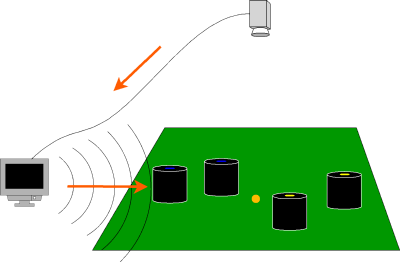
\includegraphics[ scale=0.5]{./liga_robocup/dataflow}
	\caption{Schemat komunikacji w  \mbox{\emph{Small Size League}}\newline(źródło: \texttt{www.robocup.org}) }
	\label{fig:comunication}
	\end{figure} 	
	\mbox{\emph{RoboCup VideoServer}} może rozpoznawać nie tylko położenie poszczególnych robotów, ale także ich orientację na
	płaszczyźnie. Jednak do tego celu niezbędne jest zastosowanie specjalnych znaczników. Każdej z drużyn przed rozpoczęciem rozgrywki zostaje przypisana para kolorów, jakie zawiera znacznik. Dzięki zastosowaniu dwóch kolorów możliwe jest nie tylko rozróżniania robotów z różnych drużyn, ale także właśnie ich orientacji.

\section{Budowa robota \label{sec:budowa_robota} w \emph{Small-size League}}
	W oficjalnym regulaminie ligi nie zostały narzucone konkretne modele robotów, które mogą brać udział w
	rozgrywkach, jednak, obserwując kolejne mistrzostwa, łatwo zauważyć, że wśród zgłaszanych drużyn dominuje jedna konstrukcja mechaniczna. Została ona zaprezentowana na  rysunkach \ref{fig:F180_budowa}.
 	\begin{figure}
	\centering
	\subfloat[]{\label{fig:F180_budowa1}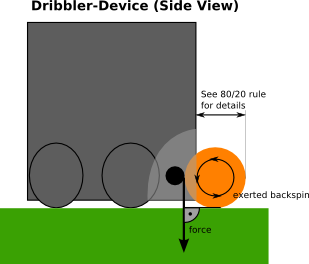
\includegraphics[ scale=0.34]{./liga_robocup/F180_budowa1}}
	\subfloat[]{\label{fig:F180_budowa2}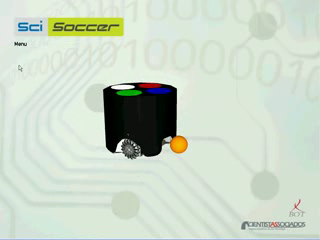
\includegraphics[ scale=0.38]{./liga_robocup/F180_budowa2}}
	\subfloat[]{\label{fig:F180_budowa3}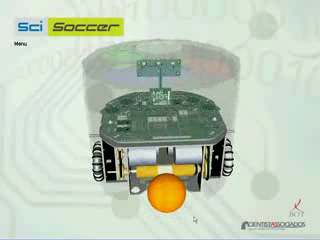
\includegraphics[ scale=0.38]{./liga_robocup/F180_budowa3}}
	\caption{Popularny model robota wykorzystywany w \mbox{lidze \emph{F180}}\newline(źródło: \texttt{www.robocup.org}) }
	\label{fig:F180_budowa}
	\end{figure}
	Podczas gry w piłkę nożną często wynika potrzeba zmiany orientacji w miejscu. W prezentowanym rozwiązaniu
	zdecydowano się na omnikierunkową bazę jezdną. Składa się ona z trzech kół szwedzkich, w tym dwóch niezależnie
	napędzanych. Koło szwedzkie posiada taką zaletę, iż dodatkowo poza obrotem wokół własnej osi umożliwia obrót
	wokół punktu styczności koła z podłożem oraz wokół osi rolek umieszczonych na kole.
	\begin{wrapfigure}{r}{0.42\textwidth}
	\vspace{-30pt}
	\begin{center}	
	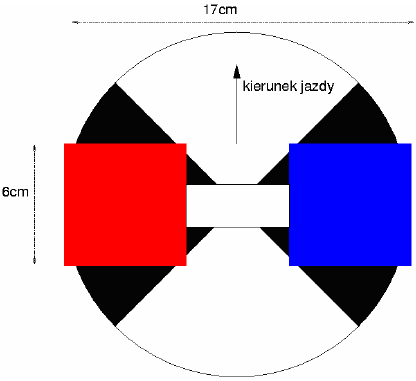
\includegraphics[width=0.38\textwidth]{./liga_robocup/znacznik}
	\end{center}
	\vspace{-10pt}	
	\caption{Znacznik umożliwiający systemowi wizyjnemu identyfikację robotów \label{fig:znacznik}}
	\vspace{-10pt}
	\end{wrapfigure}
	Dzięki zastosowaniu takiego rozwiązania uzyskano w pełni holonomiczną budową robota.
	Robot biorący udział w rozgrywkach musi być zdolny do prowadzenia piłki. Zastosowana konstrukcja jest wyposażona w urządzenie do dryblowania widoczne na rysunkach \ref{fig:F180_budowa1} oraz \ref{fig:F180_budowa3}. 
	Zbudowane jest ono z walca nadającego piłce wsteczną rotację, przez co nie odbija się ona od robota, a także nie traci on nad nią kontroli w momencie hamowania lub obracania się.
	W regulaminie rozgrywek dopuszczono do stosowania jedynie urządzenia do dryblowania 
	działające na piłkę siłą
	prostopadłą do podłoża rys.~\ref{fig:F180_budowa1} (we wcześniejszych latach w użyciu były  urządzenia, w których obracany walec był umieszczony pionowo).

	Ostatnim ważnym elementem, w który musi być wyposażony robot, jest znacznik (rys.~\ref{fig:znacznik}).
	Znajduje się on w takim miejscu, aby kamera umieszczona centralnie nad boiskiem mogła go zarejestrować (przykrywa robota od góry).
	Znaczniki umożliwiają systemowi wizyjnemu określenie, do której drużyny należy dany robot, a także poprawne rozpoznanie jego pozycji, orientacji oraz prędkości
	na boisku.

